 \providecommand{\main}{../../..}
\documentclass[\main/main.tex]{subfiles}
\begin{document}
\subsection{Esercizio 1}
Dato il seguente problema di PL:

\begin{figure}
  \begin{align*}
    \min z = 2x_1 - 3x_2   \\
    -3x_1 + 2x_2 & \leq 12 \\
    -x_1 + 2x_2  & \geq 0  \\
    x_2          & \leq 5  \\
    5x_1 + 2x_2  & \leq 30 \\
    x_1          & \in \R  \\
    x_2          & \geq 0
  \end{align*}
  \caption{Esercizio 1}
\end{figure}

\begin{enumerate}
  \item Si disegni la regione ammissibile e si evidenzi il vertice ottimo per via grafica, riportando il valore di z e di tutte le variabili del modello.
  \item Si ricavi per via grafica per quali valori di $c_1$, ora pari a $2$, la \textbf{composizione} della base ottima non cambia.
  \item Si risolva mediante gli scarti complementari il duale del problema.
\end{enumerate}

\subsection{Soluzione esercizio 1}

\subsubsection*{Identifico soluzione ottima}

\begin{figure}
  \begin{subfigure}{0.49\textwidth}
    \dddgraph{x_2}{x_1}{0}{5}{-4}{5}{-17}{-3*y+2*x<=12&&-y+2*x>=0&&x<=5&&5*y+2*x<=30}{2*y -3*x}
    \caption{Il vertice ottimo ha coordinate $\bmx = \rnd{\frac{3}{2},5}$}
  \end{subfigure}
  \begin{subfigure}{0.49\textwidth}
    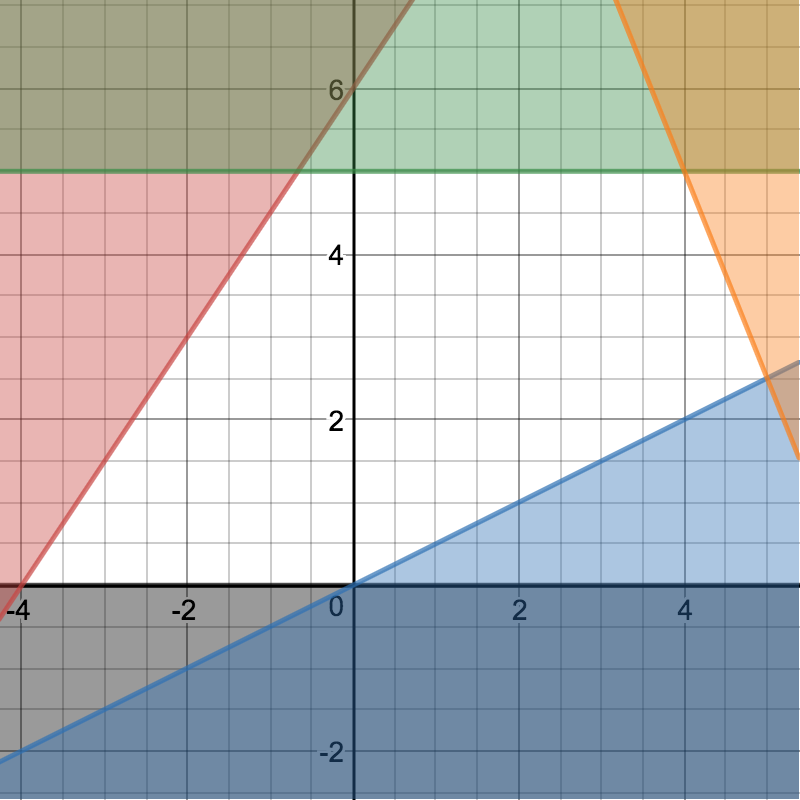
\includegraphics[width=0.9\textwidth]{2016_06_20}
    \caption{Regione di ammissibilità del problema}
  \end{subfigure}
  \caption{Vertice ottimo del problema di minimo}
\end{figure}

\subsubsection*{Riporto variabili}

\begin{align*}
  z   = -\frac{49}{3}, \quad
  x_1 = -\frac{2}{3} , \quad
  x_2 = 5            , \quad
  s_1 = 0            , \quad
  s_2 = \frac{28}{3} , \quad
  s_3 = 0            , \quad
  s_4 = \frac{50}{3} , \quad
\end{align*}
\subsubsection*{Determino il valore di $c_1$}
Variare il valore di $c_1$ può portare la soluzione ottima in $\rnd{-4,0}$ o in $(4,5)$:

\begin{figure}
  \begin{subfigure}{0.49\textwidth}
    \[
      -\frac{2}{3}c_1 -15 = -4c_1 \Rightarrow c_1 = \frac{9}{2}
    \]
    \caption{Determino il valore massimo del costo $c_1$}
  \end{subfigure}
  \begin{subfigure}{0.49\textwidth}
    \dddgraph{x_2}{x_1}{0}{5}{-4}{5}{-20}{-3*y+2*x<=12&&-y+2*x>=0&&x<=5&&5*y+2*x<=30}{9/2*y -3*x}
    \caption{Sostituendo $c_1\geq\frac{9}{2}$ la soluzione ottima si sposta in $\bmx=\rnd{-4, 0}$}
  \end{subfigure}
  \begin{subfigure}{0.49\textwidth}
    \[
      -\frac{2}{3}c_1 = 4c_1 \Rightarrow c_1 = 0
    \]
    \caption{Determino il valore minimo del costo $c_1$}
  \end{subfigure}
  \begin{subfigure}{0.49\textwidth}
    \dddgraph{x_2}{x_1}{0}{5}{-4}{5}{-20}{-3*y+2*x<=12&&-y+2*x>=0&&x<=5&&5*y+2*x<=30}{ -3*x}
    \caption{Sostituendo $c_1\leq0$ la soluzione ottima si sposta in $\bmx=(4,5)$}
  \end{subfigure}
  \caption{Analisi di sensitività}
\end{figure}

\subsubsection*{Costruisco problema duale}
\begin{align*}
  \max 12y_1 +5y_3 + 30y_4           \\
  -3y_1 -y_2 +5y_4         & = 2     \\
  2y_1 + 2y_2 + y_3 + 2y_4 & \leq -3 \\
  y_2                      & \geq 0  \\
  y_1, y_3, y_4            & \leq 0
\end{align*}
\subsubsection*{Scarti complementari}
\[
  \begin{cases}
    x_1 (-3y_1 -y_2 +5y_4-2) = 0          \\
    x_2 (2y_1 + 2y_2 + y_3 + 2y_4 +3) = 0 \\
    y_1 (-3x_1 + 2x_2 - 12) = 0           \\
    y_2 (-x_1 + 2x_2) = 0                 \\
    y_3 (x_2 - 5) = 0                     \\
    y_4 (5x_1 + 2x_2 - 30) = 0
  \end{cases}
  \Rightarrow
  \begin{cases}
    -3y_1 -2 = 0      \\
    2y_1 + y_3 +3 = 0 \\
    y_2  = 0          \\
    y_4  = 0
  \end{cases}
  \Rightarrow
  \begin{cases}
    y_1 = -\frac{2}{3} \\
    y_3= -\frac{5}{3}  \\
    y_2  = 0           \\
    y_4  = 0
  \end{cases}
\]
Sostituisco nella funzione obbiettivo e verifico che $z = z_D = -\frac{49}{3}$.
\end{document}